\subsection{QWM-Agent}\label{sec:qwm_agent}

\textit{Primary author: Alois Bachmann}

\subsubsection{Planning with World Models}

\textit{Primary author: Alois Bachmann}

Our initial approach to planning explored whether a learned world model could improve a Bomberman agent by predicting the consequences of candidate actions before they were executed in the environment. In particular, we implemented a JEPA-inspired latent dynamics model. Rather than predicting the complete next observation at the pixel (or in this case board-state) level, the model predicts a compact latent representation of the future state. Next to this representation, we also predict the value and reward for this future state using separate heads based on a candidate action. 

As an alternative to the previously explained DynaQ in Section~\ref{sec:dyna_method}, we used the world model for planning rather than as a source of synthetic training data. For this we utilized the reward and value heads to predict the return of a candidate action sequence. Candidate action sequences were generated with a genetic algorithm and evaluated by rolling them out in the learned latent dynamics model. The highest-scoring sequence determined the action executed in the real environment. 

This kind of planning was inspired by the paper on hierarchical world models \cite{zhang2026hwm}. In this paper they propose this kind of planning as an efficient way to find the best trajectory in a complex environment. In the paper this was extended with sub-goals and one main goal latent state that should be reached by the model. 

If we think about goal definitions in the Bomberman environment we can set a few example goals: The first one being the simplest one that the agent is the only thing left on the board. The problem with this goal is that this goal might lie a few hundreds steps into the future. At this point the world model has probably hallucinated a lot which makes a simulated path to that goal (even with subgoals) very inaccurate. 

The second possibility would be to define local goals which are more reachable (e.g.: collecting the nearest coin). A problem that would appear is that if we tell the model to only focus on one goal the agent might collect the coin very efficiently but does not look out for bombs placed by enemies and because of that it gets blown up in the next turn. So we would have to also implement the goal of safety and maybe enemy killing and also crate destruction and also make all of that very efficiently and so on. But when we have these different goals which one should we prioritize? We would have to weigh them and give the model a positive feedback if it achieves one of these goals and a negative one if he is failing in one of the goals. In other words: We need rewards and values (what is the ability to achieve different goals soon). 

This is why we use the value and reward heads to evaluate different candidate action sequences. By using this method we assumed that a higher value and reward for a given action sequence is closer to the final goal and lower reward and value is further away from it.

Using this method we can use a trained world-model to try and find the best action sequence. We do this (as proposed in the paper LeWorldModel \cite{maes2026leworldmodelstableendtoendjointembedding}) using a genetic algorithm like procedure: We sample a certain number of random action sequences text them out, take the best few and mutate them with one another to find the best action sequence. We mutate multiple times. The mutation step is the generation, the planning depth the internal simulation horizon of the world model and the population size the amount of different action sequences sampled.

\begin{figure}[!h]
     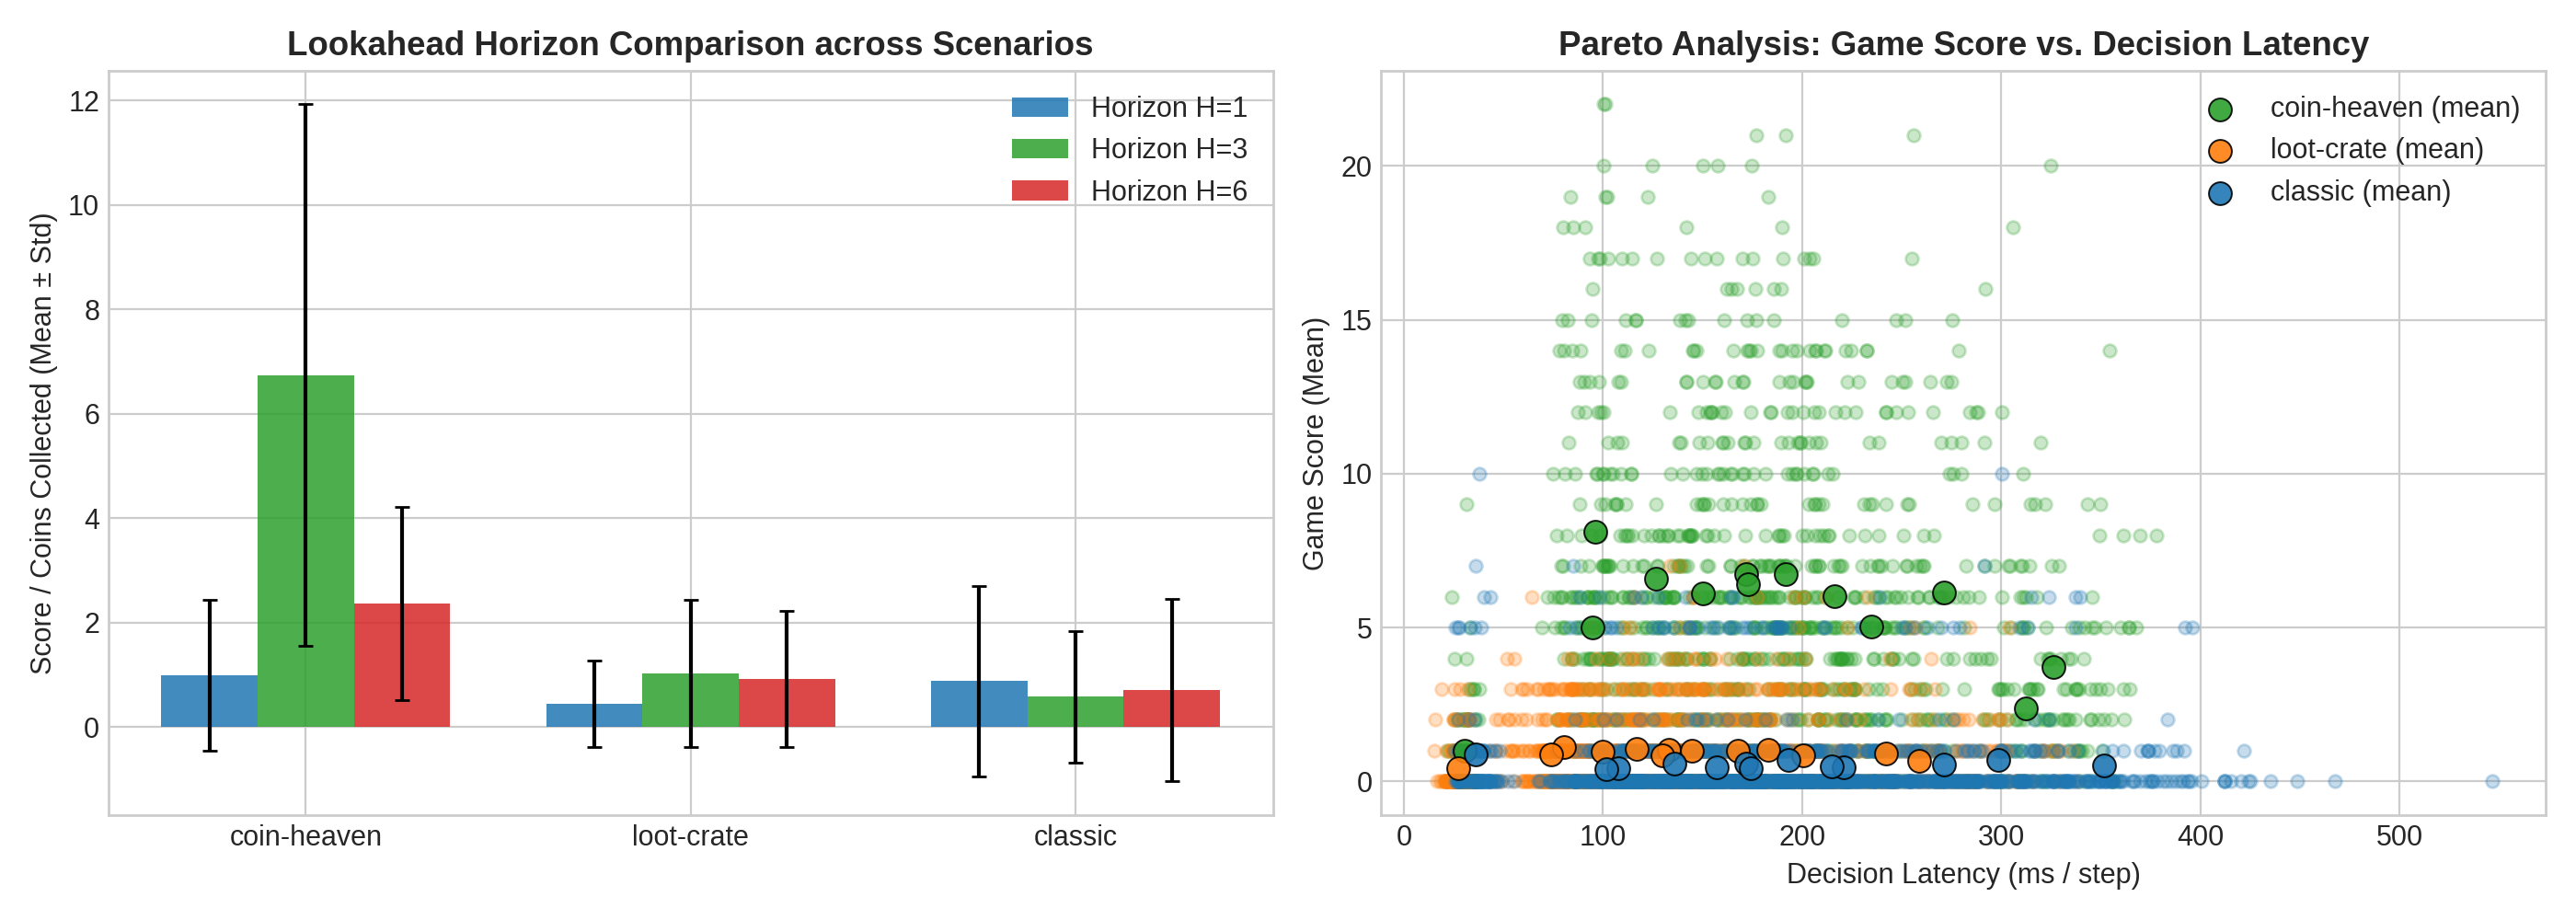
\includegraphics[width=0.96\columnwidth]{figures/ga_scenario_comparison_and_pareto.png}
     \caption{Latent planning results with pure world model with genetic algorithm and random initial action sequence sampling. Shortened environment time of max. 80 steps and no enemy agents.}
     \label{fig:pure_planning}
\end{figure}

The first thing that is visible in this plot is that we clearly have diminishing returns from long horizon planning and also long computational time. This initially seems counter-intuitive. Because we would think that if the agent can plan further into the future it would act more intelligently. 
This behavior is mainly caused by two things: 

\begin{enumerate}
    \item Not enough planning: We plainly just do not have the ability to sample enough action sequences inside our 500ms time limit to find the actual best route for a long horizon of 6 steps.
    \item Compounding world model error: Because the world model is not perfect it creates a shift in what the actual next latent representation will be every imagination step. So a small error at a low horizon can quickly compound into a very high error in longer horizons.
\end{enumerate}

Regarding the second problem: one option to improve this is that we could sample our predicted latent state using a gaussian distribution so that we do not have one deterministic state and rather a statistical one. A further improvement could be even using more binned latent representation where we decouple the information of the different bins with a new loss so that every bin only translates one information. This prevents us from mixing errors. A similar idea is used in the DreamerV3 architecture which was also tested as an option as a planning world model basis \cite{hafner2023dreamerv3}. But even with these improvements we were only able to reduce this problem and not eliminate it.

The other problem is even bigger. Because we have this hard time constraint we will only ever be able to try a set number of different action sequence and mutate them only so much. Because of this we will be stuck with sub-optimal performance. We can actually see this in figure \ref{fig:pure_planning}. We seem to be able to find reasonable action sequences for the coin-heaven but as soon as we get to the loot-crate scenario the performance degrades significantly and is not viable as a competitive agent.

This is why we need another architecture because this architecture seems to be not reasonable for the Bomberman environment. (At least not with our available resources. It may be that one can achieve better results with longer and more complex training but we were not able to get this architecture to work.)

Because we primarily have to fix the planning-complexity problem we can maybe think of sampling or pruning our action sequence space more efficiently. This is why we wanted to use a policy based action sequence sampling method. The idea behind such a method would be that we train a base reinforcement learning agent which we would train in the first step to be good in the environment already and then change the architecture where we hook into an inbetween-output to use this then to predict future representations. We then would use our base agent trained without planning in the main environment to efficiently choose next actions based on our current planning step.

While we were working on this architecture we had the luck that a paper was published right on time (on the 17th of August 2026) that was also trying to make this approach work. We therefore used this paper as a basis for our further production and then also final agent \cite{dong2026qwm}.

\subsubsection{Q-Learning with World Models}

\textit{Primary author: Alois Bachmann}

The basic idea of this agent is grounded in the paper Q-Learning with World Models \cite{dong2026qwm}. This paper describes an architecture of multiple cleverly interconnected models to achieve a policy based planning architecture. It uses one backbone agent model that learns a policy in the real environment so that it gathers a good understanding of the behaviour and physics of objects in different scenarios and take good actions based on one state. The second model is the actual world model that uses the outputs of the agents encoder model to predict the encoded state of the next time step based on some action choosen by the agent. In the original paper a big pretrained vision model was used as the vision encoder. We are not able to use such a model due to resource and time limits. Therefore we will have to train the encoder together with all the other parts of the model.

The final planning method presented in the paper is a tree search algorithm. It utilizes the ability of the model to predict q-values and rewards for every action in future time steps to efficiently prune non-promising paths to only retain a set amount of feasible paths as the final output. 

In the following we will present how we used and modified this architecture to solve the bomberman environment.

\subsubsection{Backbone model (Dueling Q-Agent)}

\textit{Primary author: Alois Bachmann}

\begin{figure}[!h]
     \includegraphics[width=0.96\columnwidth]{figures/stage1_dqn_agent.pdf}
     \caption{Backbone DQN-Agent architecture.}
     \label{fig:dqn_agent}
\end{figure}

The first thing we train is the backbone agent on its own, without a world model and without planning. Figure~\ref{fig:dqn_agent} shows this. The idea is that if this agent is already decent at picking an action from one state, we can later use those action scores to prune the search instead of trying action sequences more or less at random, which is what we were stuck with in the genetic algorithm.

The agent is a duelling Q-agent. There is a global value head and an action specific value head. The global head says how good the state is in general, and the action head says how much better or worse one action is compared to the others in that same state. We add those together to get the action scores and then just select the highest one as the action. This is the normal duelling split. It is useful here because a lot of states in bomberman are just bad no matter what you do (you are already standing in a blast) while the difference between the six actions is still what we actually have to learn.
\begin{equation}
Q(s, a) = V(s) + \left(A(s, a) - \frac{1}{|\mathcal{A}|} \sum_{a' \in \mathcal{A}} A(s, a')\right).
\end{equation}

The encoder is two things that get fused. The first is a cnn visual encoder of the whole game state, with different channels for different informations (walls, crates, coins, bombs, agents, and so on). The second is a deterministic state extractor. This one calculates things that we do not want the cnn to have to figure out on its own, like if the agent is standing in danger and in which direction the next coin is and so on. Both of these get fused into one state. This fused state is what we call the world representation.

The world representation is then passed into the value heads. So the q-values are not computed from the raw board, they are computed from this already mixed representation. Later the world model also reads from exactly this vector.

Specifically, the cnn has 4 layers ($32 \to 64 \to 64 \to 32$ channels) taking a 10-channel $17 \times 17$ grid of the board, and the deterministic feature extractor calculates 33 hand-crafted values like shortest paths to coins and crates, blast escape directions, and neighbor obstacles. They fuse through a linear layer into a 256-dimensional vector $z_t$.

We train this across a 4-stage curriculum of 12,800 rounds: starting with coin collecting in \texttt{coin-heaven}, then crate bombing in \texttt{loot-crate}, then passive opponents, and finally classic against three rule-based agents. On classic against rule-based agents it actually collects coins decently: it gets $2.66$ to $2.82$ coins per round ($29.6\%-31.5\%$ of all coins) and reaches a mean score between $3.02 \pm 2.0$ and $4.46 \pm 3.4$, with a win rate of $30.0\%$ to $46.0\%$. But the problem is that it is completely greedy. It only looks at the immediate next step. So it drops a bomb because bombing a crate gives a reward, but it does not check if it can actually walk away from the bomb over the next four ticks before it explodes. Because of this the suicide rate is horribly high: between $0.84$ and $0.88$ suicides per round, and it only survives $4.0\%$ to $6.0\%$ of the games (averaging around $115.8$ to $136.2$ steps before blowing itself up). This is the agent without any look-ahead, so these numbers are the baseline for everything we add afterwards. We then use this as a backbone for the next step.

\subsubsection{World model}

\textit{Primary author: Alois Bachmann}

\begin{figure}[!h]
     \includegraphics[width=\columnwidth]{figures/stage2_world_model.pdf}
     \caption{World model architecture inserted into the DQN-Agent.}
     \label{fig:world_model}
\end{figure}
\begin{figure*}[!h]
  \includegraphics[width=\textwidth]{figures/stage3_planning.pdf}
  \caption{Planning architecture utilizing the DQN-Agent and the World model.}
  \label{fig:planning}
\end{figure*}

We then train a world model to predict the next state (or in some cases states) going from one fused latent state and a selected action. Figure~\ref{fig:world_model} shows where this sits inside the DQN-Agent. The fused state and the action go into a world model trunk. The trunk predicts a world information vector, and from that vector we predict the actual things we care about with seperate heads.

These are:
\begin{enumerate}
    \item the reward gotten in that world state
    \item a value prediction of that latent world
    \item $\Delta z$, the fused state difference from the previous fused latent state to the next one
\end{enumerate}

The third one is the important design choice. If we asked the model to predict the full latent vector every time it would have to re-predict walls and coins that did not even move. With $\Delta z$ it only has to predict the changes, and the next fused state is just the old one plus that difference. This is also how we get more than one step. We add the predicted difference, treat that as the new fused state, and do the same thing again. The problem is of course that a small error in $\Delta z$ gets added again at the next step, which is the same compounding problem we already had with the earlier world model.

We also train a legal action prediction head. This head predicts which actions are legal to take in that predicted state. We use this later for prunning of invalid action sequences. We cannot just take the legal actions from the current real board and keep them for the whole rollout, because after one step a tile can be blocked, or a bomb can be ticking, or the agent might already have a bomb down. So the legal set has to be predicted together with the state.

This model is trained in different steps. In the beginning we freeze the dqn agent and really only train the world model. The dqn already produces a fused state that means something, and if we train both at the same time that state keeps moving and the world model is chasing a target that changes underneath it. We train the different heads and the world model trunk so it can accuratly predict the effects of one action on the environment.

Specifically, the 256-dimensional fused state $z_t$ is concatenated with a 6-dimensional one-hot action vector $a_t$, giving a 262-dimensional input. The trunk is two linear layers with hidden dimension 256 and \texttt{DynActivation}. In Stage 0 ($s_0$, 900 rounds), we set \texttt{dqn\_frozen = 1}. With the dqn frozen, the transition residual loss drops from above $0.45$ to below $0.05$ very quickly. After that, we train both together across the remaining curriculum stages.

\begin{figure}[!h]
     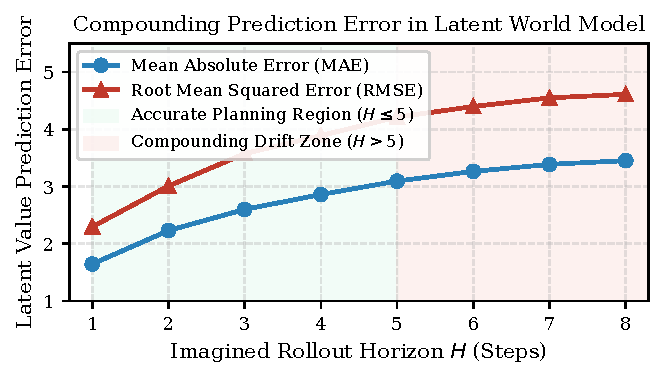
\includegraphics[width=\columnwidth]{figures/world_model_horizon_error.pdf}
     \caption{Latent world model prediction error (MAE and RMSE) across recursive rollout horizons $H=1$ through $8$ on held-out validation trajectories. Compounding drift degrades value accuracy beyond $H>5$.}
     \label{fig:world_model_horizon_error}
\end{figure}

To see how bad the compounding error gets, we measured the prediction error of this model across rollout horizons $H=1$ to $8$ on validation trajectories (Figure~\ref{fig:world_model_horizon_error}). At step 1 the prediction is quite accurate: the Mean Absolute Error ($\text{MAE}$) is $1.65$ and Root Mean Squared Error ($\text{RMSE}$) is $2.30$. But because small errors in $\Delta z$ add up every step, by step 8 the error compounds to $\text{MAE} = 3.45$ and $\text{RMSE} = 4.61$. This is why we cannot just roll out 10 or 15 steps into the future, and why we discount future steps heavily with $\lambda = 0.08$.

\subsubsection{Tree-search Planning}

\textit{Primary author: Alois Bachmann}

Using the trained world model and dqn agent we then finally go over to planning. Figure~\ref{fig:planning} shows this. Planning is working in the way where we test at every possible turn every possible action. This is viable and is fine with efficiency because the dqn agent already predicts q-values for all the available actions. We do not have to sample random sequences and then mutate them, like in the genetic algorithm. The backbone already tells us which actions look good in the state we are currently imagining.

This way a tree is created because we recursivly, after one action, once again try every action and so on. Because this would be horribly inefficient we only retain the best $b$ action sequences on the fly and then use these ends of the tree to look further into the future. Like this we only really have a number of max $b$ simulations into the future at the same time. This is the fix for the planning-complexity problem from before. We still do not search the whole tree, but the paths we drop are the ones the q-values already say are bad, not paths we happened to not sample.

Over the action sequences we accumulate all q-values and rewards and then choose the action sequence with the highest accumulated q-value. Because both the dqn agent and the world model have q value heads we add those weighted for every step. We then also have an exponential decay of the q-values so that predictions for the model in the farther future are less important (because of the problem of compounding bias otherwise). A q-value at step 8 is not worth the same as a q-value at step 1 for action choosing.

We then use our legal action head to filter out found trajectories with illegal moves so they do not affect the performance of our agent. A sequence can have a high accumulated value and still contain a move into a wall or into a blast that the world model imagined badly. Those sequences are just removed.

We also add another small model that specifically penalizes full action sequences to filter out loops and unnecessary bomb or wait moves. This model is called just before choosing the final action to take in the next move. The tree search looks at one step at a time, so a loop or a useless wait can survive for a while if every single step looks ok on its own. The small model instead sees the whole sequence and can explicitly penalize multiple actions at once. 

We train this part of the model after the world model is able to predict proper future states and the dqn agent produces good local results. We train the model on random horizons of 1 through 8 so that the planning is both accurate short term and long term. If we only trained on horizon 8 the next step (which is the only action we actually execute) would be undertrained. If we only trained on horizon 1 we would be back to the backbone agent and the bomb timer, which only pays off a few steps later, would not show up in the search.

Specifically, we use beam size $b=18$, keeping the top $K=3$ branches per root action. We score each candidate action sequence $a_{0:H-1}$ by summing the root Q-value, discounted rewards, discounted value predictions, and subtracting the sequence penalty:
\begin{equation}
\begin{aligned}
S(a_{0:H-1}) = Q(s_0, a_0) &+ \sum_{t=0}^{H-1} \lambda^t \left[\hat{r}_t + \alpha_{vq} \hat{V}(\hat{z}_{t+1})\right] \\
&- P(a_{0:H-1}).
\end{aligned}
\end{equation}
We set $\lambda = 0.08$ so that uncertain future predictions cannot override what the agent sees right now, scale future values with $\alpha_{vq} = 0.16$, and subtract the penalty $P(a_{0:H-1})$ with weight $0.25$. The small penalty model is a 3-layer MLP with 5,893 parameters (~23 KB) using LayerNorm and \texttt{DynActivation}. It takes a 56-dimensional trajectory summary that tracks corridor oscillations, U-turns, idle waits, and walking into bomb blasts. We trained it with 40 epochs of supervised regression on penalty data from Optuna ($R^2 = 0.99996$, validation MSE $1.2 \times 10^{-4}$), and then 240 rounds of reinforcement fine-tuning in mixed classic games.

\begin{figure}[!h]
     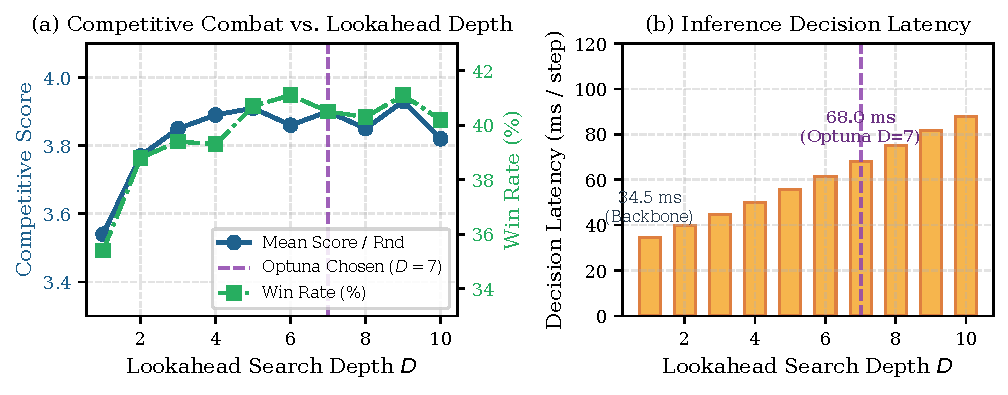
\includegraphics[width=\columnwidth]{figures/qwm_depth_sweep.pdf}
     \caption{Systematic planning horizon sweep ($D=1\dots 10$) across 1,000 rounds per depth on matched random seeds. (a) Competitive score and win rate stay high across $D=5\dots 7$, with $D=7$ chosen by Optuna for long-term evaluations. (b) Decision latency scales from 34.5 ms to 87.9 ms, remaining well within the 500 ms limit.}
     \label{fig:qwm_depth_sweep}
\end{figure}

To pick the best search depth $D$, we ran a systematic depth sweep from $D=1$ to $10$ over 1,000 rounds per depth (Figure~\ref{fig:qwm_depth_sweep}). Without planning ($D=0$) the agent is basically suicidal. Once we turn on planning, win rate jumps from around $4\%$ to over $40\%$. The score peaks locally around $D=5$ with $3.91 \pm 0.20$ (win rate $40.7\%$, $55.5$ ms latency). But when we ran an Optuna hyperparameter optimization trial over the full planning pipeline, the optimizer selected depth $D=7$ as the best overall configuration (score $3.90$, win rate $40.5\%$, $68.0$ ms latency). $D=7$ looks two steps further ahead than $D=5$ while still staying far below our 500 ms time limit. Because the Optuna trial chose $D=7$, we used $D=7$ as our fixed planning depth for all long-term evaluations and tournament duels. Beyond $D \ge 7$, the score starts dropping slightly while the latency goes up to $87.9$ ms, because the compounding error in deeper world model rollouts starts to hurt.
